\documentclass{beamer}
%\mode<presentation>
\usepackage[utf8]{inputenc}
\usepackage[magyar]{babel}
\usetheme{CambridgeUS}
\usecolortheme{dolphin}
\usepackage{amsmath,amssymb,amsfonts, bm}
\usepackage{mathpazo}
\usepackage{graphicx,tabularx,epsfig}
\usepackage[compatibility=false]{caption}
\usepackage{subcaption}
\usepackage{rotating}

\DeclareGraphicsExtensions{.pdf,.png,.jpg,.svg}

\setbeamertemplate{itemize items}[square]
\setbeamertemplate{enumerate items}[square]

\definecolor{Red}{RGB}{190,0,0}
\definecolor{Blue}{RGB}{0,0,190}




\title[Numerikus hidrodinamika]{Nagyenergiás nehézion-ütközések numerikus hidrodinamikai modellezése}
\author[Bagoly Attila]{Bagoly Attila\\ ELTE TTK Fizika BSc, 3. évfolyam \vspace{0.5cm}\\  Témavezető:\\ Csanád Máté}
\date[2015.04.29.]{Bolyai Kollégium, Szakszeminárium \\ 2015.04.29.}
\institute[ELTE]{ELTE TTK Atomfizikai tanszék}
\begin{document}

\begin{frame}
  \titlepage
\end{frame}


\section{Bevezető}
\begin{frame}
\frametitle{Bevezető}

  \begin{itemize}
    \setlength{\itemsep}{14pt}

\item<1-> Nehézion ütközések: nagy energiasűrűség $\rightarrow$  kvark szabadsági fokok
\item<1-> Ősrobbanás: univerzum kvarkok és gluonok ``őslevese''
%\item<2-> Új ismeretek: kvark-gluon plazma vizsgálata
\item<1-> Kísérleti tapasztalat (2005): tökéletes folyadék
\item<1-> Nagy hatáskeresztmetszetek, gyors termalizáció $\rightarrow$ statisztikus fizika %Nagy hatáskeresztmetszetek, rövid szabad úthossz, gyors termalizáció: statisztikus fizika
\end{itemize}

\begin{minipage}{0.62\textwidth}
\begin{itemize}
\item<1-> Kezdeti eloszlás: aszimmetriák $\rightarrow$ kifagynak a részecskék eloszlásában
\end{itemize}

\end{minipage}
\begin{minipage}{0.37\textwidth}
\begin{center}
\begin{figure}
\centering
	\includegraphics<1->[scale=0.24]{pic/p2}
\end{figure}
\end{center}
\end{minipage}




\end{frame}

\begin{frame}
\frametitle{Motiváció}

Kvark-gluon plazma folyadékszerű viselkedésének következtében:
\vspace{10pt}
	\begin{itemize}
		  \setlength{\itemsep}{8pt}
		\item<1-> hogyan hatnak különböző effektusok az aszimmetriák időfejlődésére
		\item<1-> analitikusan nem kezelhető effektusok
	\end{itemize}
\vspace{20pt}
$\Longrightarrow$ Numerikus hidrodinamika: realisztikus modell QGP-re, de minden effektus hatása keveredik
\vspace{20pt}


$\Longrightarrow$ Kezdőfeltétel: legyen közel létező analitikus megoldásokhoz, de realisztikusabb modellt adjon
\end{frame}

\begin{frame}
\frametitle{Tartalom}
\begin{enumerate}
  \setlength{\itemsep}{16pt}
\item<1-> Hidrodinamika egyenletei
\item<1-> Numerikus módszer
\item<1-> Kód tesztelése
\item<1-> Nemrelativisztikus eredmények
\item<1-> Relativisztikus eredmények
\end{enumerate}

\end{frame}

\section{Hidrodinamika egyenletei}
\begin{frame}
\frametitle{Hidrodinamika egyenletei}
\begin{itemize}
\item<1-> Nemrelativisztikus hidrodinamika:
\begin{itemize}
\item<1-> Anyagmegmaradás:\quad \begin{large}$\dfrac{\partial \rho}{\partial t} + \bm{\nabla}\rho\bm{v}=0$\end{large}
\item<1-> Impulzusmegmaradás:\quad \begin{center}\begin{large}$\rho\Big(\dfrac{\partial \bm{v}}{\partial t}+(\bm{v\nabla})\bm{v}\Big)=-\bm{\nabla}p +\mu\Delta\bm{v}+\Big(\zeta+\dfrac{\mu}{3}\Big)\bm{\nabla}(\bm{\nabla v})+\bm{f}$\end{large}\end{center}
\item<1-> Energiamegmaradás: \quad\begin{large}$\dfrac{\partial \varepsilon}{\partial t}+\bm{\nabla}\varepsilon\bm{v}=-p\bm{\nabla v}+\bm{\nabla(\sigma v)}$\end{large}
\item<1-> $\rho$ anyagsűrűség, $\bm{v}$ sebességmező, $\varepsilon$ energiasűrűség, $p$ nyomáseloszlás
\end{itemize}

\item<1-> Relativisztikus hidrodinamika:
\begin{Large}
\begin{center}$T^{\mu\nu}=\big(\varepsilon+p\big)u^\mu u^\nu-pg^{\mu\nu},\quad \partial_\mu T^{\mu\nu}=0$\end{center}
\end{Large}
\begin{itemize}
\item<1-> $T^{\mu\nu}$ energia-impulzus tenzor, $u^\mu$ négyes-sebesség, $g^{\mu\nu}$ metrikus tenzor
\end{itemize}

\item<1-> Állapotegyenlet:\quad \begin{large}$\varepsilon=\kappa(T)p\quad$\end{large} ($\kappa=1/c_s^2$, $\kappa=3/2$ id. gáz)

\item<1-> Advekciós forma: $\partial_t Q(\rho, \varepsilon, \bm{v})+\partial_x F(Q)=0$ $\quad$ ($F$ fluxus)

\end{itemize}
\end{frame}

\begin{frame}
\frametitle{Általános relativitáselmélet röviden}
\begin{itemize}
  \setlength{\itemsep}{16pt}

\item Ívelemnégyzet: $ds^2=dx_\mu dx^\mu=g_{\mu\nu} dx^\mu dx^\nu$
\item Konnexió: $w(x+dx)^\mu=\overline{v(x)}^\mu=v(x)^\mu-\Gamma_{\nu\lambda}^\mu v^\nu dx^\lambda$
\item Deriválás: $\nabla_\mu v^\nu=\partial_\mu v^\nu +\Gamma^{\nu}_{\lambda\mu}v^\lambda$
\item Riemann-geometria: $\Gamma = \partial g$
\item Görbület: $\Delta v_\mu =\frac{1}{2}\Delta f^{\nu\lambda}R^{\rho}_{\mu\nu\lambda}v_\rho$, $[\nabla_\mu,\nabla_\nu]v_\lambda = R^{\rho}_{\lambda\mu\nu}v_\rho$, $R=g^{\mu\nu}R_{\mu\rho\nu}^\rho$
\item Tehát görbületet jellemző skalár: $R\propto \partial \Gamma \propto \partial^2 g$
\end{itemize}

\end{frame}

\begin{frame}
\frametitle{Általános relativitáselmélet röviden}
\begin{itemize}
  \setlength{\itemsep}{16pt}
\item Anyag görbíti a téridőt:
\begin{equation*}
S[g]=\frac{1}{c}\int d^4x \sqrt{-g}\Big(\mathcal{L}_M+\frac{c^4}{16\pi G}R\Big) 
\end{equation*}
\item Ennek variációja:
\begin{equation*}
\delta S=\frac{1}{c}\int d^4x \sqrt{-g}\Big(\frac{1}{2}T^{\mu\nu}-\frac{c^4}{16\pi G}\big(R^{\mu\nu}-\frac{1}{2}Rg^{\mu\nu}\big)\Big)\delta g_{\mu\nu}
\end{equation*}
\item Einstein egyenlet:
\begin{equation*}
R^{\mu\nu}-\frac{1}{2}Rg^{\mu\nu}=\frac{8\pi G}{c^4}T^{\mu\nu}
\end{equation*}

\item Kovariáns divergenciát kiszámolva:

\begin{equation*}
\nabla_\mu T^{\mu\nu}=0
\end{equation*}

\end{itemize}


\end{frame}


\begin{frame}
\frametitle{Honnan jönnek a relativisztikus hidrodinamika egyenletei?}

\begin{itemize}
  \setlength{\itemsep}{20pt}

\item Folyadék: csak belső energia: \begin{large}$\mathcal{L}_M=\varepsilon$\end{large}
\item Hatás "anyagi" része: $S_M= \int \frac{d^4x}{c}\sqrt{-g}\mathcal{L}_M$
\item Energia-impulzus tenzor: $\delta S_M=\int \frac{d^4x}{c}\sqrt{-g}\frac{1}{2}T_{\mu\nu}\delta g^{\mu\nu}$
\item Mitől függ a belső energia? 
\end{itemize}

\end{frame}



\begin{frame}
\frametitle{Termodinamika}
\begin{itemize}
  \setlength{\itemsep}{16pt}

\item Sűrűségek $\epsilon=\frac{E}{V}$ (energia), $\sigma = \frac{S}{V}$ (entrópia), $n=\frac{N}{V}$ (szám)
\item Termodinamika első főtétele (felhasználva az Euler egyenletet és Gibbs-Duham relációt):
\begin{equation*}
d\epsilon=Td\sigma +\mu dn
\end{equation*} 

\item Entrópiasűrűség metrikus tenzor szerinti deriváltja?

\item Legyen $s=\frac{S}{N}$ $\rightarrow$ ezt könnyebb deriválni metrika szerint

\item Főtétel átírva:
\begin{equation*}
d\epsilon=\frac{\epsilon+p}{n}dn+nTds
\end{equation*}

\item Tehát \begin{large}$\varepsilon(n,s)$\end{large}
\end{itemize}

\end{frame}

\begin{frame}
\frametitle{Energia-impulzus tenzor meghatározása}
\begin{itemize}
\item Variáljunk: 
\begin{equation*}
\delta S=\int \frac{d^4 x}{c}\bigg[\epsilon \delta \sqrt{-g}+\sqrt{-g}\bigg(\frac{\partial\epsilon}{\partial n}\delta n+\frac{\partial \epsilon}{\partial s}\delta s\bigg)\bigg]
\end{equation*}
\item Mi a fajlagos entrópia variációja?
\begin{itemize}
\item $s=S/N$
\item Részecskeszám nem függ a metrikától!
\item A rendszer entrópiája sem!
\item $\delta s= 0$
\end{itemize}
\item Mi a számsűrűség variációja?

\begin{equation*}
\delta N = \delta \int n dV_0= \delta \int \frac{d^4x}{d\tau c}\sqrt{-g}n=0\Rightarrow \delta\bigg(\frac{n\sqrt{-g}}{d\tau}\bigg)=0
\end{equation*}
\begin{equation*}
\Rightarrow  \delta ln\bigg(\frac{n\sqrt{-g}}{d\tau}\bigg)=0 \Rightarrow \frac{\delta n}{n}=\frac{\delta(d\tau)}{d\tau}-\frac{\delta\sqrt{-g}}{\sqrt{-g}}
\end{equation*}

\end{itemize}


\end{frame}

\begin{frame}
\frametitle{Energia-impulzus tenzor meghatározása}
\begin{itemize}
\item Ívelem variációja:
\begin{equation*}
\delta(d\tau)=\frac{1}{c}\delta\sqrt{ds^2}=\frac{1}{c}\frac{1}{2ds}\delta(ds^2)=\frac{1}{2c^2 d\tau}\delta(g_{kl}dx^kdx^l)
\end{equation*}
\begin{equation*}
\Rightarrow \frac{\delta(d\tau)}{d\tau}=\frac{1}{2c^2}\frac{dx^k}{d\tau}\frac{dx^l}{d\tau}\delta g_{kl}=\frac{1}{2c^2}u^ku^l\delta g_{kl}
\end{equation*}

\item Determináns mátrixelem szerinti deriváltja: $\frac{\partial A}{\partial A_{kl}}=A(A^{-1})_{kl}$
 \begin{large}$\Rightarrow$\end{large}
\begin{equation*}
\delta g = g g^{kl}\delta g_{kl}
\end{equation*}

\item Jacobi-determináns variációja:
\begin{equation*}
\delta \sqrt{-g}=\frac{1}{2\sqrt{-g}}(-g)g^{kl}\delta g_{kl}=\frac{\sqrt{-g}}{2}g^{kl}\delta g_{kl}
\end{equation*}
\begin{equation*}
\Rightarrow \delta n=\frac{n}{2}(\frac{u^ku^l}{c^2}-g^{kl})\delta g_{kl}
\end{equation*}
\end{itemize}

\end{frame}

\begin{frame}
\frametitle{Energia-impulzus tenzor meghatározása}
\begin{itemize}
\item A hatás variációja:
\begin{equation*}
\delta S=\int \frac{d^4 x}{c}\bigg[\epsilon\frac{\sqrt{-g}}{2}g^{kl}\delta g_{kl}+\sqrt{-g}\frac{\varepsilon+p}{n}\frac{n}{2}(\frac{u^ku^l}{c^2}-g^{kl})\delta g_{kl}\bigg]
\end{equation*}
\begin{equation*}
\Rightarrow\delta S=\int \frac{d^4 x}{c}\frac{\sqrt{-g}}{2}\bigg[\epsilon g^{kl}+(\epsilon+p)\bigg(\frac{u^ku^l}{c^2}-g^{kl}\bigg)\bigg]\delta g_{kl}
\end{equation*}
\item Ideális folyadék energia-impulzus tenzor: $T^{kl}=(\epsilon+p)\frac{u^ku^l}{c^2}-pg^{kl}$
\item Minkowski-téridőben az egyenletek:
\begin{equation*}
\partial_{\mu}T^{\nu\mu}=0
\end{equation*}
\end{itemize}

\end{frame}








%\begin{frame}
%\frametitle{Multipole solution}
%  \begin{minipage}{0.39\textwidth}
%    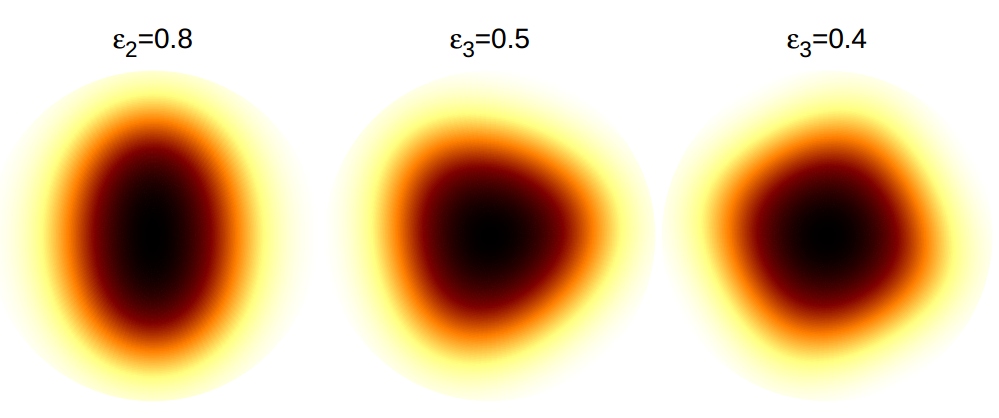
\includegraphics[scale=0.16]{pic/a1}

%    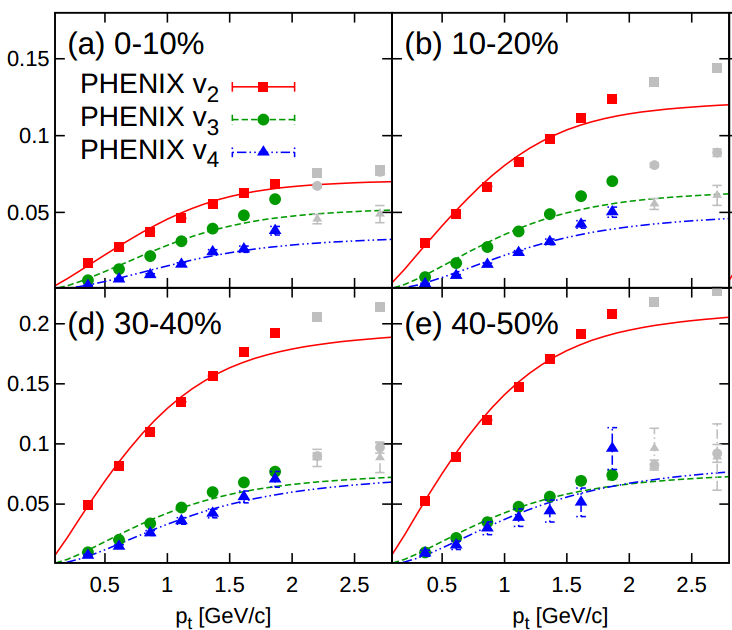
\includegraphics[scale=0.2]{pic/a2}
%  \end{minipage}
%  \begin{minipage}{0.60\textwidth}
%  \begin{itemize}
%\item New exact solution of relativistic hydrodynamics by Máté Csanád and András Szabó, published Phys.Rev. C90 (2014) 054911
%\item The solution in cylindrical coordinates:
%$u^\mu=\frac{x^\mu}{\tau}$, $n=n_f\big(\frac{\tau_f}{\tau}\big)^3\nu(s)$, $p=p_f\big(\frac{\tau_f}{\tau}\big)^{3+3/\kappa}$
%\item Where $\tau$ is the coordinate-proper time, $\tau_f$ is the freeze-out proper time
%\item The s scale variable with any asymmetries 
%$s=\frac{r^N}{R^N}\Big(1+\epsilon_{N}\cos N\phi\Big)+\frac{z^N}{R^N}$
%\item That's a solution if $R=u_tt$
%\end{itemize}
%  \end{minipage}
%\end{frame}

\section{Numerikus módszer}
\begin{frame}
\frametitle{Numerikus módszer}
\begin{itemize}
  \setlength{\itemsep}{5pt}

\item<1-> Transzverz sík kitüntetett:  $2+1$ dimenziós egyenletek
\item<1-> Numerikus megoldás: diszkretizáció $\leftarrow$ véges térfogat módszer
%\item<3-> Véges térfogat módszer: mennyiségek átlaga rácspont körül
\item<1-> Probléma: fluxusok a rácspontok között
\item<1-> Instabilitás: perturbáció amely rácspontokban nulla $\rightarrow$ CFL feltétel
\item<1-> 2 térdimenziót bonyolult $\rightarrow$ operátor szétválasztás
\item<1-> Viszkozitás: ideális fluxus + viszkózus fluxus $\leftarrow$ operátor szétválasztás
\end{itemize}
\begin{center}
\includegraphics<1->[scale=0.19]{pic/f1}
\end{center}
\end{frame}

\subsection{Operátorok felbontása}
\begin{frame}
\frametitle{Operátorok felbontása}
\begin{large}
\begin{equation*}
\partial_t u = Au+Bu
\end{equation*}

\begin{equation*}
u(t+\Delta t)=e^{\Delta t(A+B)}u(t)
\end{equation*}


\begin{equation*}
u_{\rm{Lie}}(t+\Delta t)=e^{\Delta tA}e^{\Delta tB}u(t)
\end{equation*}

\begin{equation*}
u_{\rm{Strang}}(t+\Delta t)=e^{\frac{1}{2}\Delta tA}e^{\Delta tB}e^{\frac{1}{2}\Delta tA}e^{\Delta tB}u(t)
\end{equation*}
\end{large}
\end{frame}

\subsection{Viszkózus hidrodinamika}
\begin{frame}
\frametitle{Viszkózus hidrodinamika}
\begin{equation*}
\partial_t Q + \partial_x F_{\rm id}(Q)+\partial_y G_{\rm id}(Q)+\partial_x F_{\rm visc}(Q,\partial Q)+\partial_y G_{\rm visc}(Q,\partial Q) = 0
\end{equation*}
\vspace{10pt}
$\Longrightarrow$ operátorfelbontás
\vspace{10pt}
\begin{itemize}
\setlength{\itemsep}{20pt}
\item<1-> Ideális lépés: $\partial_t Q + \partial_x F_{\rm id}(Q)+\partial_y G_{\rm id}(Q)=0\rightarrow Q^{\rm id},\partial Q^{\rm id}$

$\rightarrow F_{\rm visc}, G_{\rm visc}$ 

\item<1-> Viszkózus lépés: $\partial_t Q + \partial_x F_{\rm visc}(Q^{\rm id},\partial Q^{\rm id})+\partial_y G_{\rm visc}(Q^{\rm id},\partial Q^{\rm id}) = 0$ 

$\rightarrow Q$ 

\end{itemize}
\end{frame}

\subsection{MUSTA}
\begin{frame}
\frametitle{MUSTA módszer}
\begin{itemize}
\item<1-> n-edik időlépésben: $Q^{(0)}_i\equiv Q^n_i$,  $Q^{(0)}_{i+1}\equiv Q^{n}_{i+1}$
\item<1-> $\ell$-edik előrejelzett fiktív értékek: $Q^{(\ell)}_{i}$, $F^{(\ell)}_{i}\equiv F\big(Q^{(\ell)}_{i}\big)$
\item<1-> Köztes érték és fluxus:
\begin{equation*}
Q^{(\ell)}_{i+\frac{1}{2}}=\frac{1}{2}\Big[Q^{(\ell)}_i+Q^{(\ell)}_{i+1}\Big]-\frac{1}{2}\frac{\Delta t}{\Delta x}\Big[F^{(\ell)}_{i+1}-F^{(\ell)}_i\Big], \quad F_M^{(\ell)} \equiv F\big(Q^{(\ell)}_{i+\frac{1}{2}}\big)
\end{equation*}

\item<1-> Korrigált cellaközi fluxus:
\begin{equation*}
F^{(\ell)}_{i+\frac{1}{2}}=\frac{1}{4}\Big[F^{(\ell)}_{i+1}+2F^{(\ell)}_M+F^{(\ell)}_{i}-\frac{\Delta x}{\Delta t}\Big(Q^{(\ell)}_{i+1}-Q^{(\ell)}_i\Big)\Big]
\end{equation*}
\item<1-> Következő előrejelzés a korrigált fluxusok meghatározásához:
\begin{equation*}
Q_i^{(\ell+1)}=Q^{(\ell)}_i-\frac{\Delta t}{\Delta x}\Big[F^{(\ell)}_{i+\frac{1}{2}}-F^{(\ell)}_i\Big]
\end{equation*}
%\begin{equation*}
%Q_{i+1}^{(l+1)}=Q^{(l)}_{i+1}-\frac{\Delta t}{\Delta x}\Big[F^{(l)}_{i+1}-F^{(l)}_{i+\frac{1}{2}}\Big]
%\end{equation*}
\item<1-> $\mathit\mathbf{{k}}$ lépés $\rightarrow$ $F_{i+\frac{1}{2}}=F_{i+\frac{1}{2}}^{(\mathit\mathbf{{k}})}$ $\Longrightarrow\; Q^{n+1}_i=Q^{n}_i-\frac{\Delta t}{\Delta x}(F_{i+\frac{1}{2}}-F_{i-\frac{1}{2}})$
\item<1-> A módszer publikálva: E. F. Toro et al, 2006, J. Comp. Phys
\end{itemize}
\end{frame}

\subsection{Kifejlesztett kód tesztelése}
\begin{frame}
\frametitle{Kód tesztelése}
\begin{itemize}
  \setlength{\itemsep}{5pt}
\item<1-> Egzakt megoldással (Csörgő et al, PhysRevC67)
\item<1-> Relatív hiba a numerikus és analitikus megoldás közt:
\begin{equation*}
\int{|\rho_{\rm{analitikus}}(t,\underline{x})-\rho_{\rm{numerikus}}(t,\underline{x})|d^2x}\bigg/\int{\rho_{\rm{analitikus}}(t,\underline{x})}d^2x
\end{equation*}
\end{itemize}
\begin{center}
%\visible<1->{$X=Y$ \qquad\qquad\qquad\qquad\qquad\qquad\qquad $X\neq Y$}
\begin{figure}[H]
	\centering
    \begin{subfigure}[b]{0.49\textwidth}
    		\includegraphics<1->[width=\textwidth]{pic/sym}
	\end{subfigure}
	\begin{subfigure}[b]{0.49\textwidth}
        	\includegraphics<1->[width=\textwidth]{pic/asym}
	\end{subfigure}
\end{figure}
\end{center}
\end{frame}

\section{Numerikus módszer}
\subsection{Relativisztikus kód tesztelése}
\begin{frame}
\frametitle{Relativisztikus kód tesztelése: Számsűrűség \\ $\kappa=2$ és $\kappa=4$}
\begin{center}
\begin{figure}[H]
	\centering
    \begin{subfigure}[b]{0.49\textwidth}
    		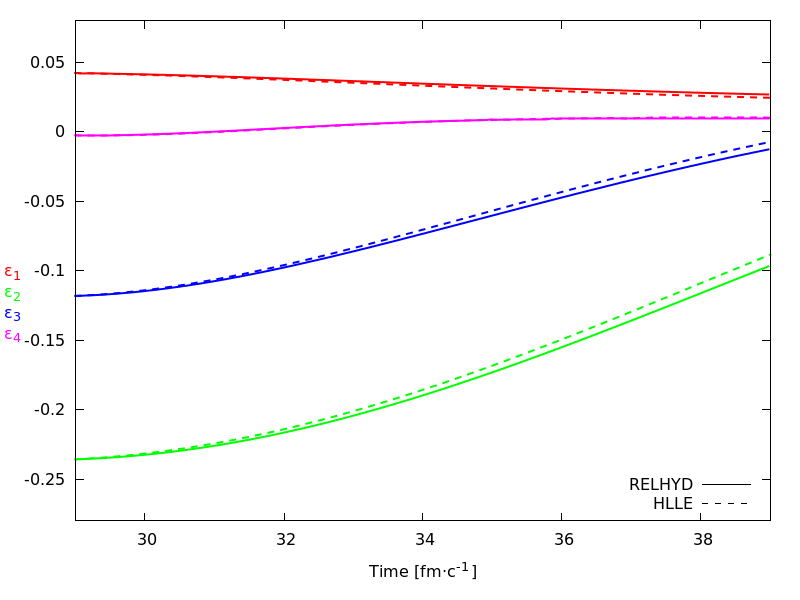
\includegraphics[width=\textwidth]{pic/res/hr_n_kappa=2}
	\end{subfigure}
	\begin{subfigure}[b]{0.49\textwidth}
        	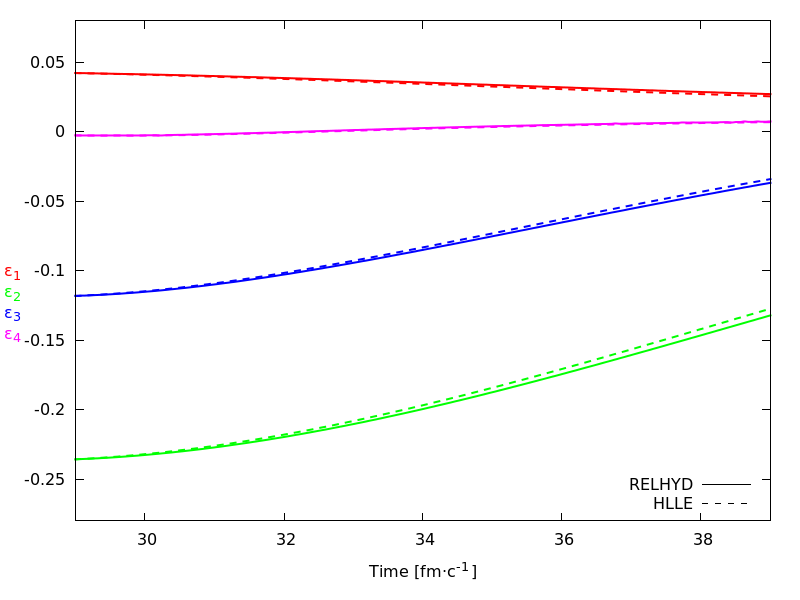
\includegraphics[width=\textwidth]{pic/res/hr_n_kappa=4}
	\end{subfigure}
\end{figure}
\end{center}
\end{frame}

\begin{frame}
\frametitle{Relativisztikus kód tesztelése: Nyomás \\ $\kappa=2$ és $\kappa=4$}
\begin{center}
\begin{figure}[H]
	\centering
    \begin{subfigure}[b]{0.49\textwidth}
    		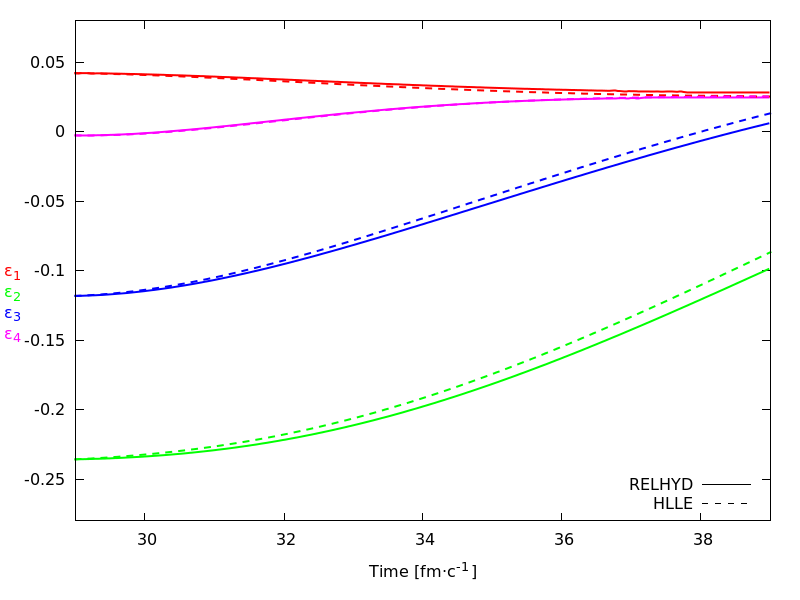
\includegraphics[width=\textwidth]{pic/res/hr_p_kappa=2}
	\end{subfigure}
	\begin{subfigure}[b]{0.49\textwidth}
        	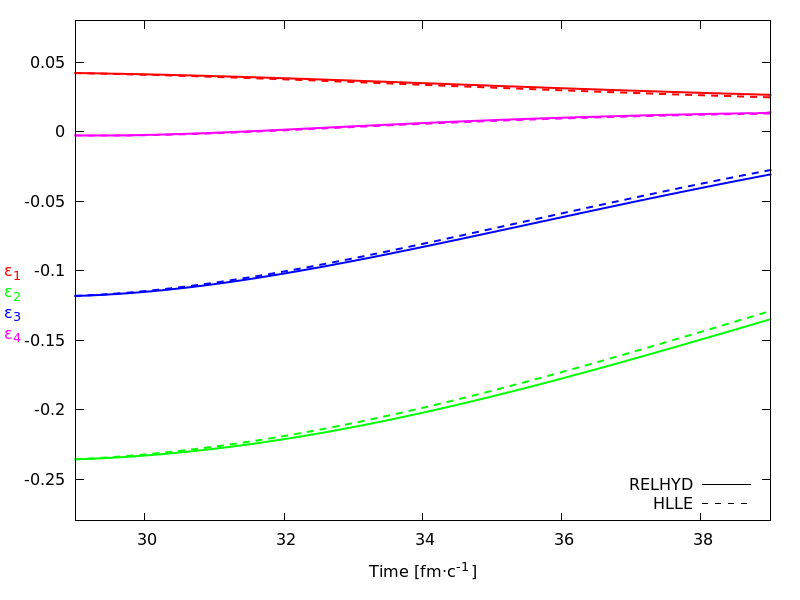
\includegraphics[width=\textwidth]{pic/res/hr_p_kappa=4}
	\end{subfigure}
\end{figure}
\end{center}
\end{frame}

\begin{frame}
\frametitle{Relativisztikus kód tesztelése: Sebességmező \\ $\kappa=2$ és $\kappa=4$}
\begin{center}
\begin{figure}[H]
	\centering
    \begin{subfigure}[b]{0.49\textwidth}
    		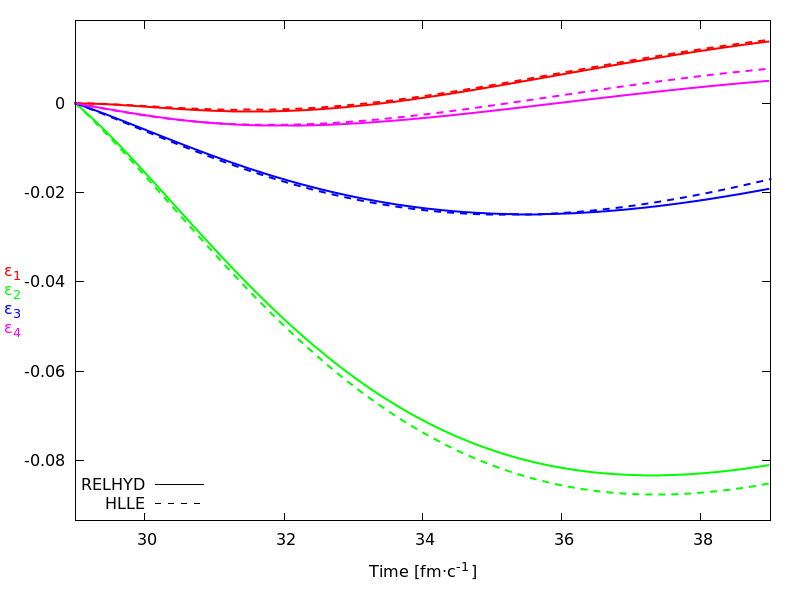
\includegraphics[width=\textwidth]{pic/res/hr_v_kappa=2}
	\end{subfigure}
	\begin{subfigure}[b]{0.49\textwidth}
        	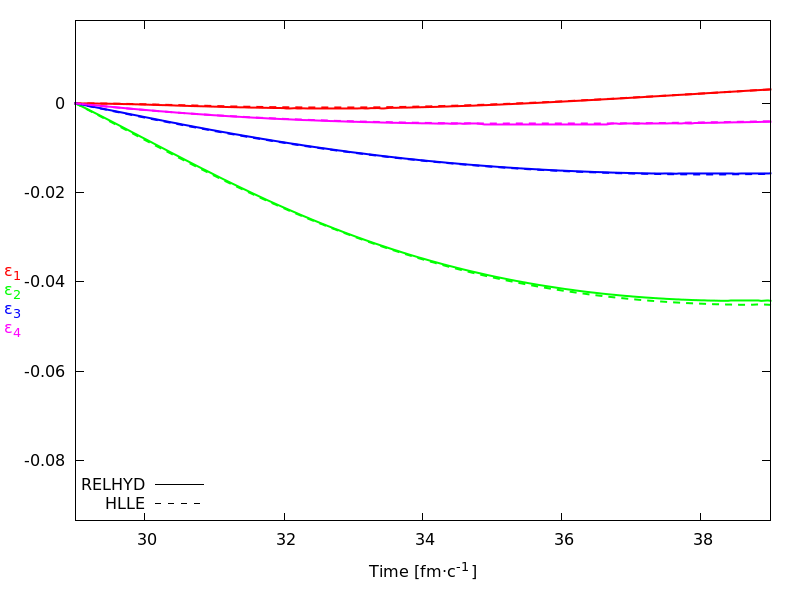
\includegraphics[width=\textwidth]{pic/res/hr_v_kappa=4}
	\end{subfigure}
\end{figure}
\end{center}
\end{frame}



\subsection{Kezdőeloszlások}
\begin{frame}
\frametitle{Kezdőfeltétel}
\begin{itemize}
  \setlength{\itemsep}{6pt}
\item<1-> Mennyiségek: helyfüggés csak skálaváltozóban, ebben szimmetria
\item<1-> Számsűrűség és nyomás \large{$\propto \exp{(-s)}$}
\item<1-> Skálaváltozó: 
\begin{equation*}
s=\frac{r^2}{R^2}\Big(1+\epsilon_2\cos(2\phi)+\epsilon_3\cos(3\phi)+\epsilon_4\cos(4\phi)\Big)
\end{equation*}
\begin{center}
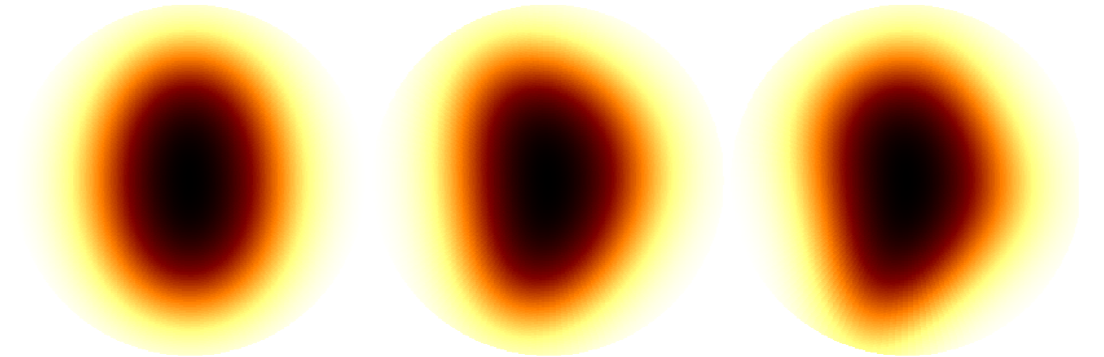
\includegraphics[scale=0.15]{pic/ic}
\end{center}
\item<1-> Sebesség: Hubble-sebességmező vagy $0$
\item<1-> Nyomásgradiens vizsgálata: \large{$p \propto \exp{(-\rm{c_p}\cdot s)}$}
\item<1-> Konstans nyomással multipólus analitikus megoldás: Csanád és Szabó, \\Phys.Rev. C90 (2014) 054911
\end{itemize}
\end{frame}

\subsection{Aszimmetria paraméterek}
\begin{frame}
\frametitle{Aszimmetriák jellemzése}
\begin{itemize}
  \setlength{\itemsep}{12pt}
\item<1-> Skálaváltozó: $s=\frac{r^2}{R^2}\big(1+\textcolor{Red}{\epsilon_2}\cos(2\phi)+\textcolor{Red}{\epsilon_3}\cos(3\phi)+\textcolor{Red}{\epsilon_4}\cos(4\phi)\big)$
\item<1-> Aszimmetriát jellemző paraméter: $\textcolor{Blue}{\varepsilon_n}=\langle \cos(n\phi)\rangle_{\rho/\bm{v}/p}$
\item<1-> $\textcolor{Blue}{\varepsilon_n}$ (most bevezetett)  $\neq$ $\textcolor{Red}{\epsilon_m}$  (kezdőfeltétel skálaváltozójában)
\item<1-> Kezdetben a $\textcolor{Blue}{\varepsilon_n}$ és $\textcolor{Red}{\epsilon_m}$ közti kapcsolatot becsülhetjük Taylor-sorfejtéssel:
\vspace{10pt}
\begin{itemize}
 \setlength{\itemsep}{8pt}
\item<1-> $\textcolor{Blue}{\varepsilon_1}=0+\textcolor{Red}{\epsilon_3}(\textcolor{Red}{\epsilon_2}+\textcolor{Red}{\epsilon_4})+\mathcal{O}(\textcolor{Red}{\epsilon^4})$
\item<1-> $\textcolor{Blue}{\varepsilon_2}=-\textcolor{Red}{\epsilon_2}+\textcolor{Red}{\epsilon_2}\textcolor{Red}{\epsilon_4}+\textcolor{Red}{\epsilon_2}\sum_{n} \textcolor{Red}{\epsilon_n^2}+\mathcal{O}(\textcolor{Red}{\epsilon^4})$
\item<1-> $\textcolor{Blue}{\varepsilon_3}=-\textcolor{Red}{\epsilon_3}+\textcolor{Red}{\epsilon_3}\sum_n \textcolor{Red}{\epsilon_n^2}+\mathcal{O}(\textcolor{Red}{\epsilon^4})$
\item<1-> $\textcolor{Blue}{\varepsilon_4}=-\textcolor{Red}{\epsilon_4}+\frac{1}{2}\textcolor{Red}{\epsilon_2^2}-\textcolor{Red}{\epsilon_4}\sum_n\textcolor{Red}{\epsilon_n^2}+\mathcal{O}(\textcolor{Red}{\epsilon^4})$
\end{itemize}
\end{itemize}

\end{frame}

\section{Nemrelativisztikus eredmények}

\subsection{Viszkozitás hatása}
\begin{frame}
\frametitle{Viszkozitás hatása}
\begin{center}
\begin{itemize}
  \setlength{\itemsep}{2pt}

\item<1-> Energiasűrűségben és  anyagsűrűségben: lassít
\begin{itemize}
\item<1-> Viszkozitás: lassítja az áramlást
\end{itemize}
\item<1-> Sebességeloszlásban: gyorsít
\begin{itemize}
\item<1-> Nagyobb,kisebb aszimmetriájú részek más erőt éreznek: különbségek gyorsan eltűnnek
\end{itemize}
\item Ábra: \large{\textcolor{red}{$\varepsilon_1$ piros}, \textcolor{green}{$\varepsilon_2$ zöld}, \textcolor{blue}{$\varepsilon_3$ kék},  \textcolor{magenta}{$\varepsilon_4$ magenta}}
\end{itemize}
\begin{figure}[H]
	\centering
    \begin{subfigure}[b]{0.49\textwidth}
    		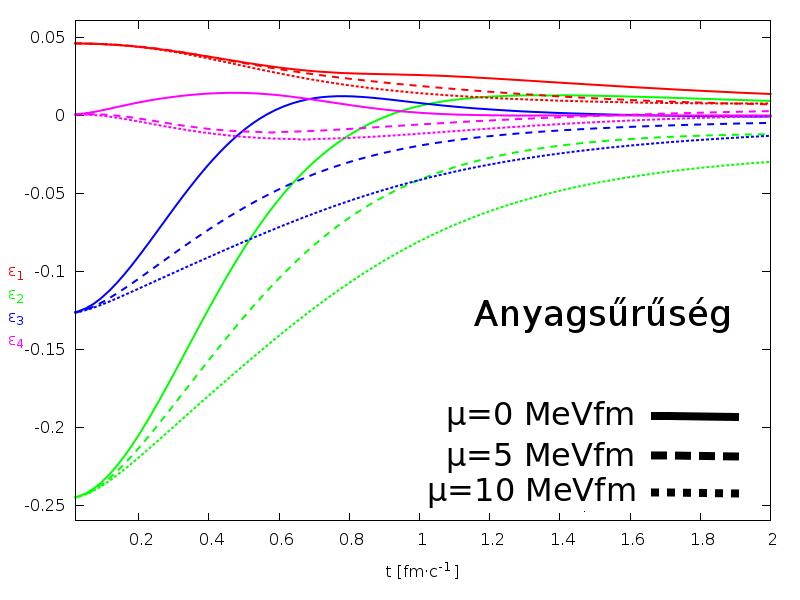
\includegraphics[width=\textwidth]{pic/res/nonrel/eps_visc_r}
	\end{subfigure}
	\begin{subfigure}[b]{0.49\textwidth}
        	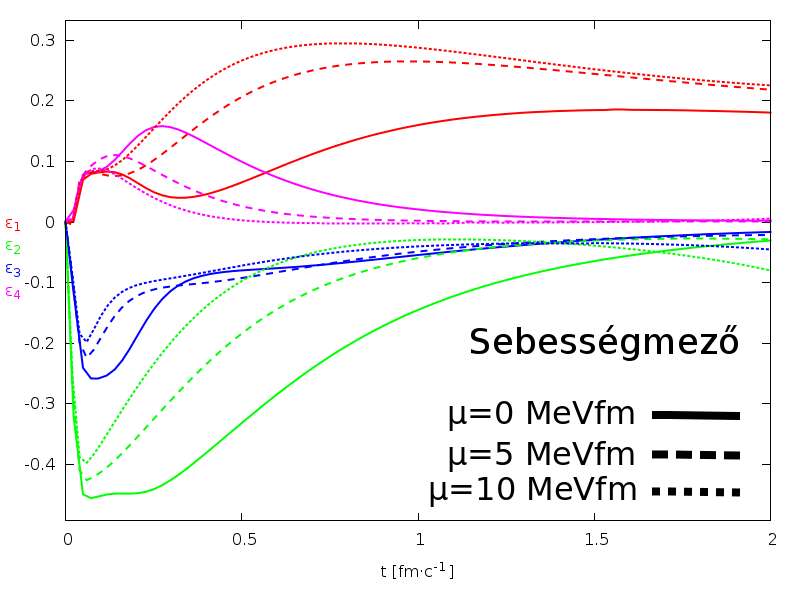
\includegraphics[width=\textwidth]{pic/res/nonrel/eps_visc_v}
	\end{subfigure}
\end{figure}
\end{center}
\end{frame}

\begin{frame}
\frametitle{Viszkozitás hatása: energiasűrűség időfejlődése}
\begin{minipage}{0.04\textwidth}
\rotatebox[origin=c]{90}{$\qquad$\scalebox{0.85}{$\mu=0\;\textnormal{MeVfm}/c$}}
\rotatebox[origin=c]{90}{\scalebox{0.85}{$\mu=10\;\textnormal{MeVfm}/c$}}
\end{minipage}
\begin{minipage}{0.95\textwidth}
\begin{center}
    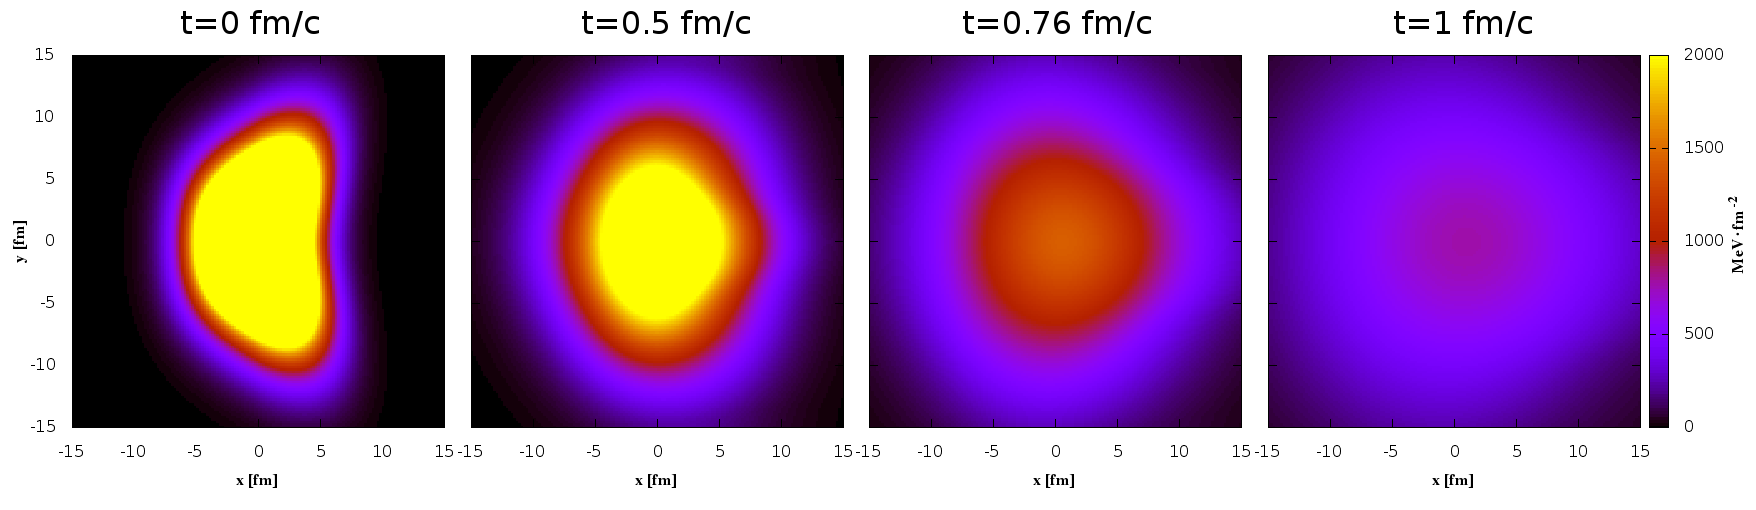
\includegraphics[scale=0.19]{pic/res/nonrel/anim/ev0}

    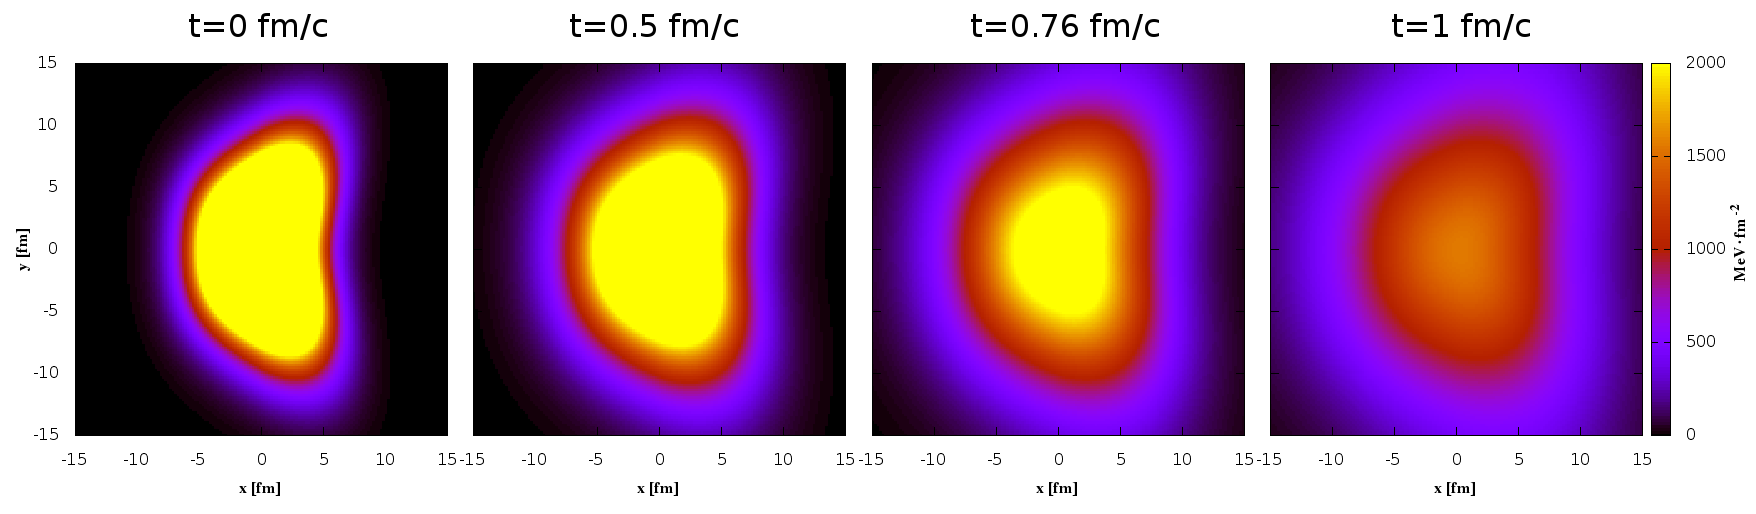
\includegraphics[scale=0.19]{pic/res/nonrel/anim/ev10}
\end{center}
\end{minipage}
\end{frame}
\begin{frame}
\frametitle{Viszkozitás hatása:  sebességeloszlás időfejlődése}
\begin{minipage}{0.04\textwidth}
\rotatebox[origin=c]{90}{$\qquad$\scalebox{0.85}{$\mu=0\;\textnormal{MeVfm}/c$}}
\rotatebox[origin=c]{90}{\scalebox{0.85}{$\mu=10\;\textnormal{MeVfm}/c$}}
\end{minipage}
\begin{minipage}{0.95\textwidth}
\begin{center}
    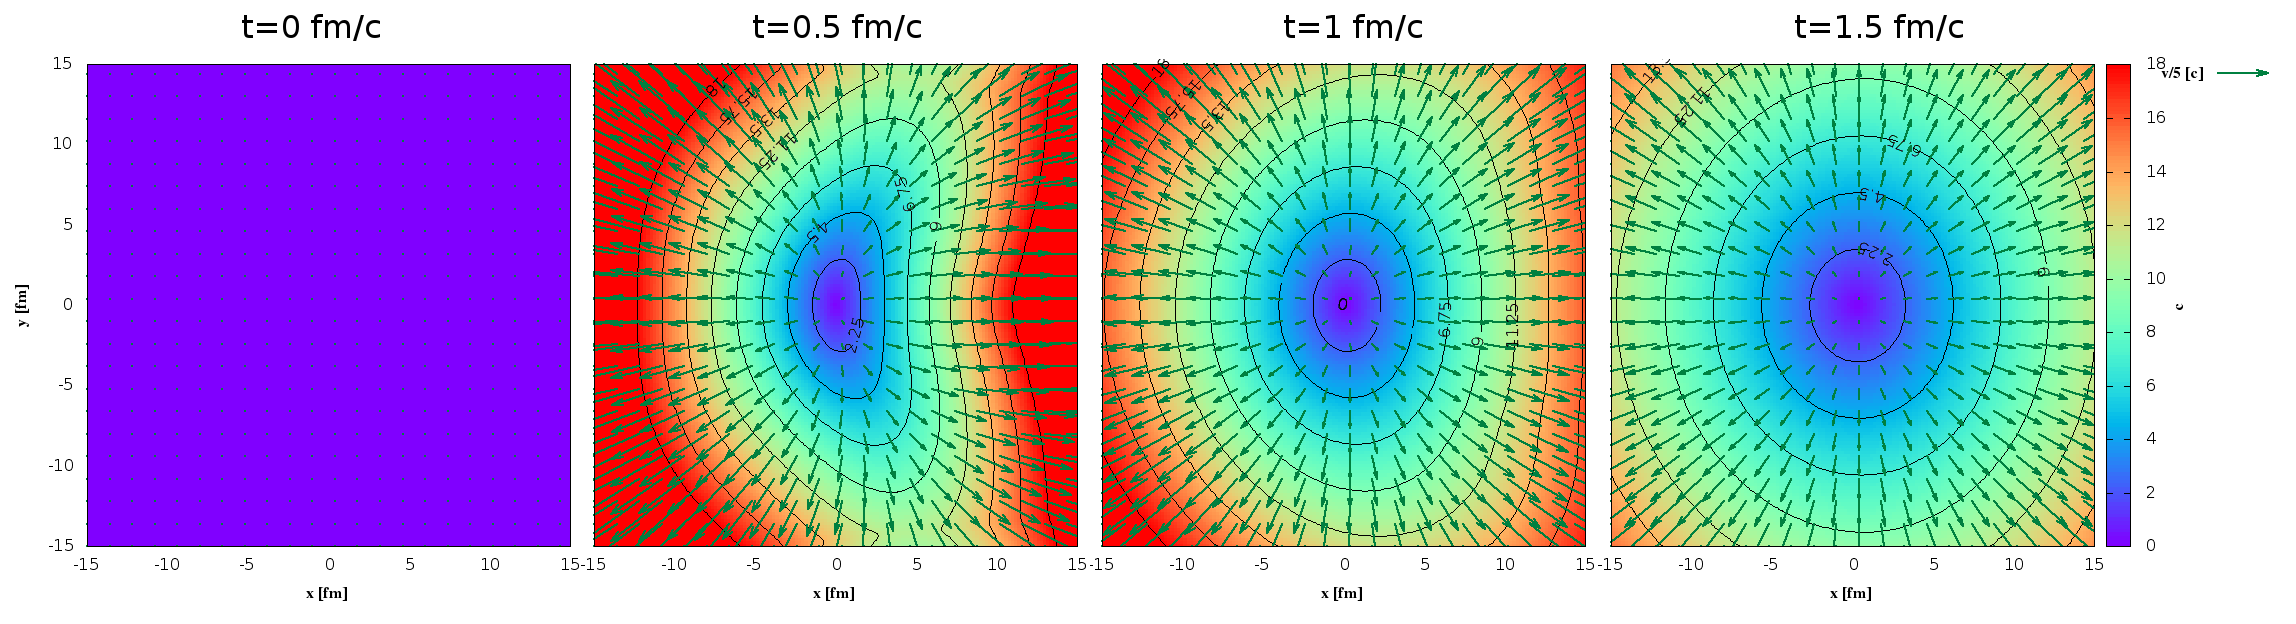
\includegraphics[scale=0.15]{pic/res/nonrel/anim/vv0}

    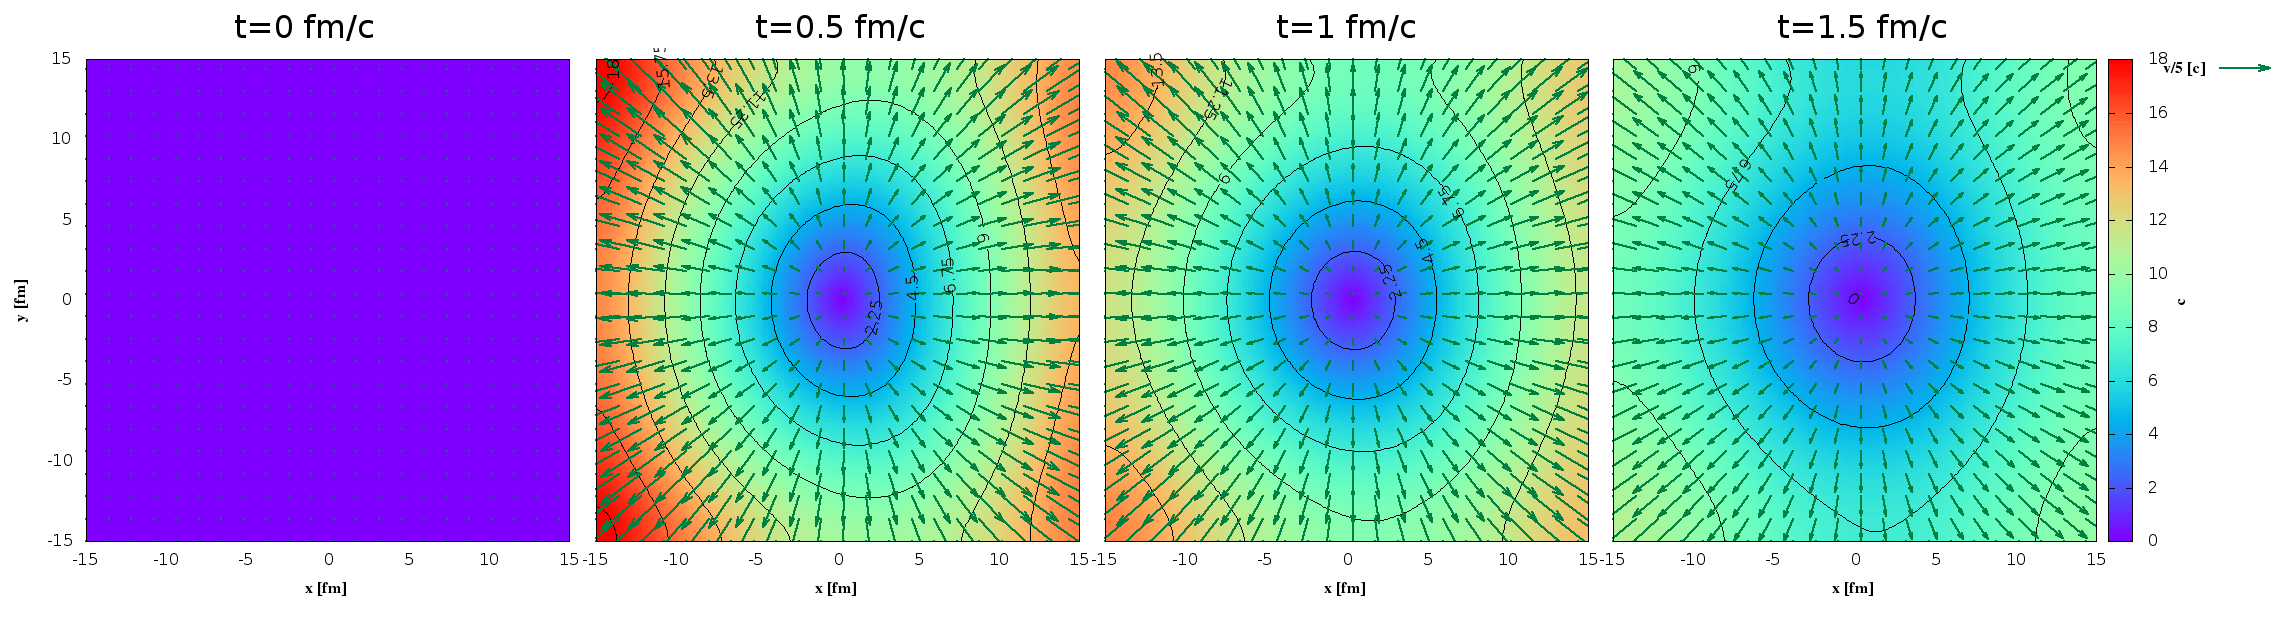
\includegraphics[scale=0.15]{pic/res/nonrel/anim/vv10}
\end{center}
\end{minipage}
\end{frame}

\subsection{Hangsebesség hatása}
\begin{frame}
\frametitle{Hangsebesség hatása}
\begin{center}
\begin{itemize}
\setlength{\itemsep}{12pt}
\item<1-> Minden eloszlásban: aszimmetriák eltűnése lassul
\vspace{8pt}
\begin{itemize}
\item<1-> Nyomáshullámok sebessége csökken $\rightarrow$ kiegyenlítődés tovább tart
\end{itemize}
\item Hangsebességek: $c_s^2=1\; \rm{vagy}\;0,4\; \rm{vagy}\; \rm{0,33}\; vagy\; \rm{0,25}$
\end{itemize}
\begin{figure}[H]
	\centering
    \begin{subfigure}[b]{0.49\textwidth}
    		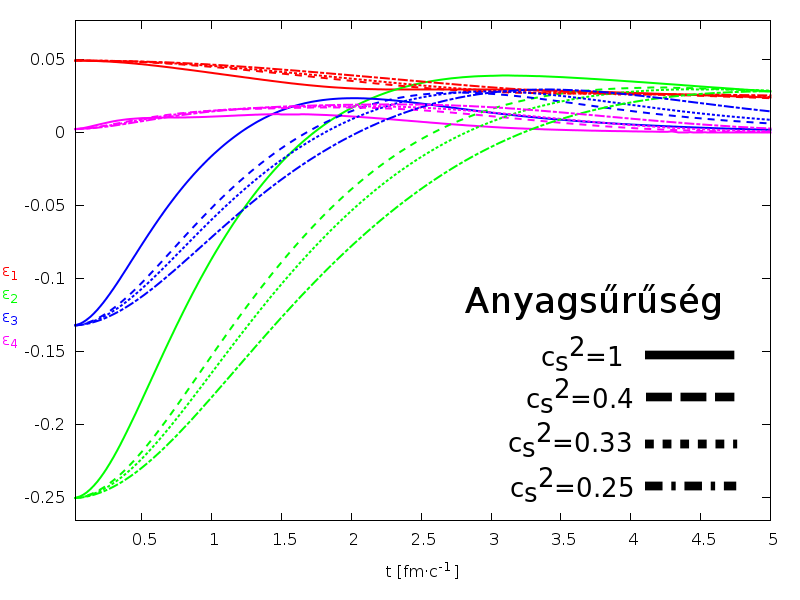
\includegraphics[width=\textwidth]{pic/res/nonrel/eps_cs2_r}
	\end{subfigure}
	\begin{subfigure}[b]{0.49\textwidth}
        	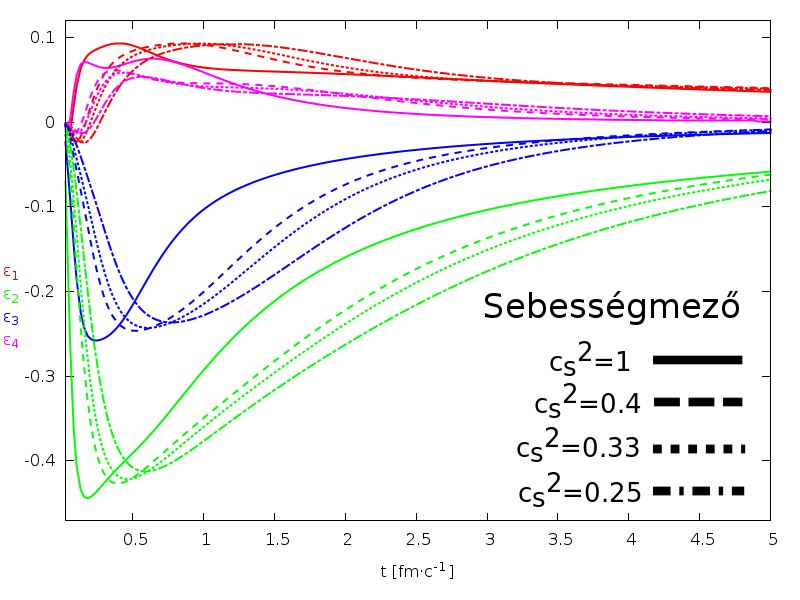
\includegraphics[width=\textwidth]{pic/res/nonrel/eps_cs2_v}
	\end{subfigure}
\end{figure}
\end{center}
\end{frame}

\subsection{Nyomásgradiens hatása}
\begin{frame}
\frametitle{Nyomásgradiens hatása}
\begin{center}
\begin{itemize}
\setlength{\itemsep}{12pt}
\item<1-> Minden eloszlásban: aszimmetriák gyorsabban eltűnnek
\begin{itemize}
\vspace{8pt}
\item<1-> Nagyobb gradiens: gyorsabb áramlás
\end{itemize}
\item<1-> Anyagsűrűség $\propto \exp{(-s)}$
\item<1-> Nyomás $\propto \exp{(-\rm{c_e}\cdot s)}$
\end{itemize}
\begin{figure}[H]
	\centering
    \begin{subfigure}[b]{0.49\textwidth}
    		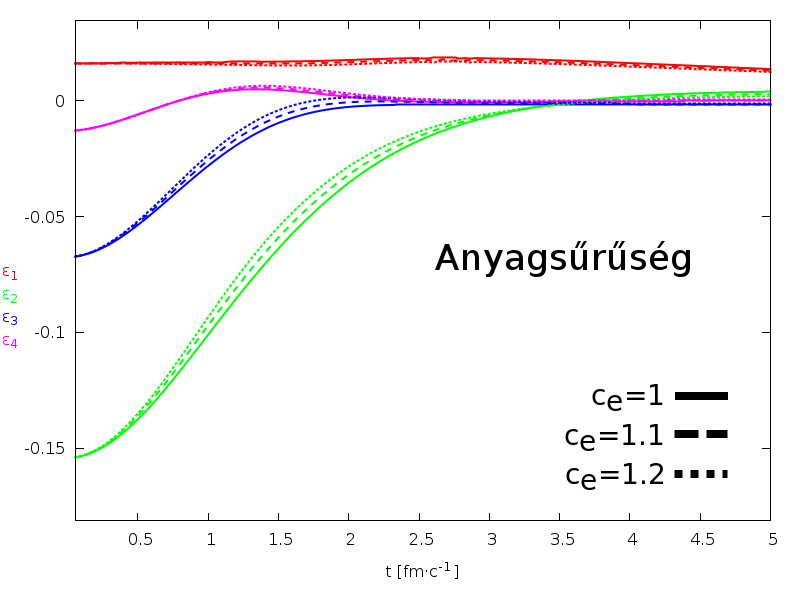
\includegraphics[width=\textwidth]{pic/res/nonrel/eps_ec_r}
	\end{subfigure}
	\begin{subfigure}[b]{0.49\textwidth}
        	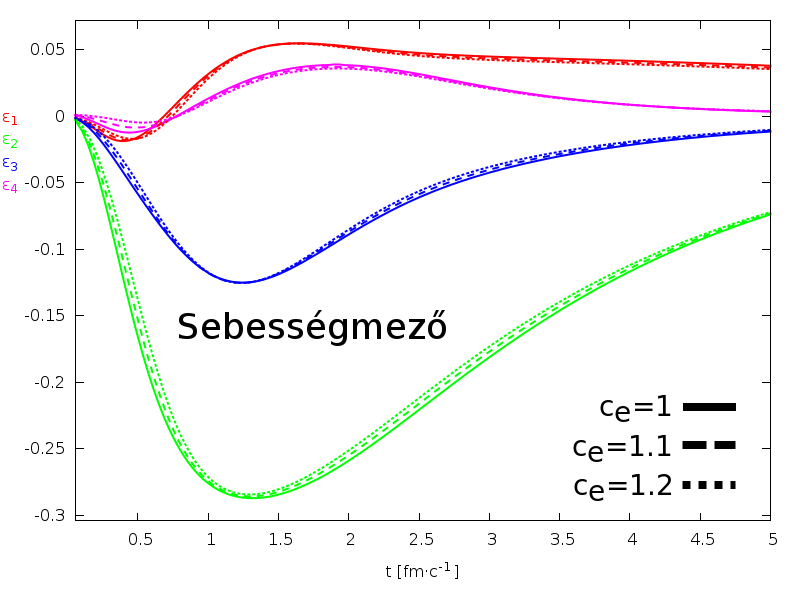
\includegraphics[width=\textwidth]{pic/res/nonrel/eps_ec_v}
	\end{subfigure}
\end{figure}
\end{center}
\end{frame}

\section{Relativisztikus eredmények}
\subsection{Hangsebesség hatása}
\begin{frame}
\frametitle{Hangsebesség hatása}
\begin{center}
\begin{itemize}
\setlength{\itemsep}{12pt}
\item<1-> Minden eloszlásban: aszimmetriák eltűnése lassul
\vspace{8pt}
\begin{itemize}
\item<1-> Nyomáshullámok sebessége csökken $\rightarrow$ kiegyenlítődés tovább tart
\end{itemize}
\item<1-> Kifagyás máskor történik!
\end{itemize}
\begin{figure}[H]
	\centering
    \begin{subfigure}[b]{0.49\textwidth}
    		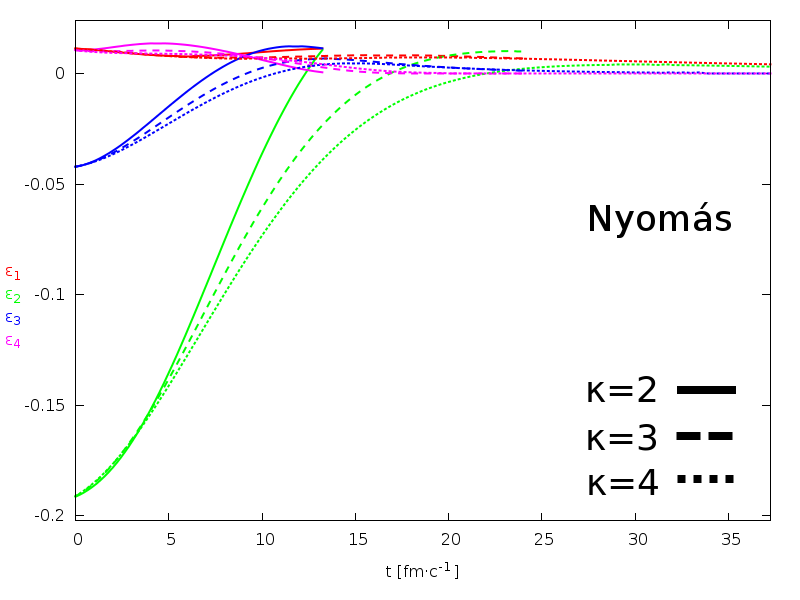
\includegraphics[width=\textwidth]{pic/res/rel/eps_kappa_p}
	\end{subfigure}
	\begin{subfigure}[b]{0.49\textwidth}
        	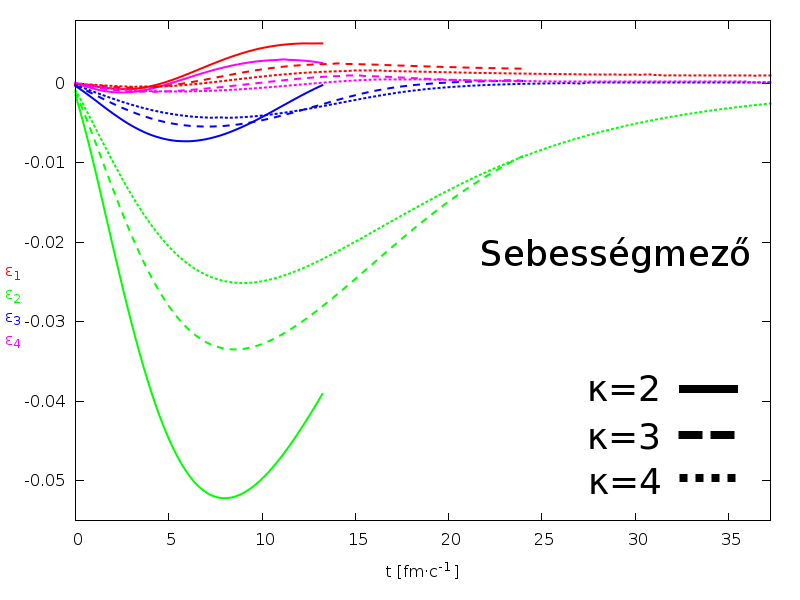
\includegraphics[width=\textwidth]{pic/res/rel/eps_kappa_v}
	\end{subfigure}
\end{figure}
\end{center}
\end{frame}

\subsection{Nyomásgradiens hatása}
\begin{frame}
\frametitle{Nyomásgradiens hatása}
\begin{center}
\begin{itemize}
\setlength{\itemsep}{12pt}
\item<1-> Minden eloszlásban: aszimmetriák gyorsabban eltűnnek
\begin{itemize}
\vspace{8pt}
\item<1-> Nagyobb gradiens: gyorsabb áramlás
\end{itemize}
\item<1-> Számsűrűség $\propto \exp{(-s)}$
\item<1-> Nyomás $\propto \exp{(-\rm{c_p}\cdot s)}$
\end{itemize}
\begin{figure}[H]
	\centering
    \begin{subfigure}[b]{0.49\textwidth}
    		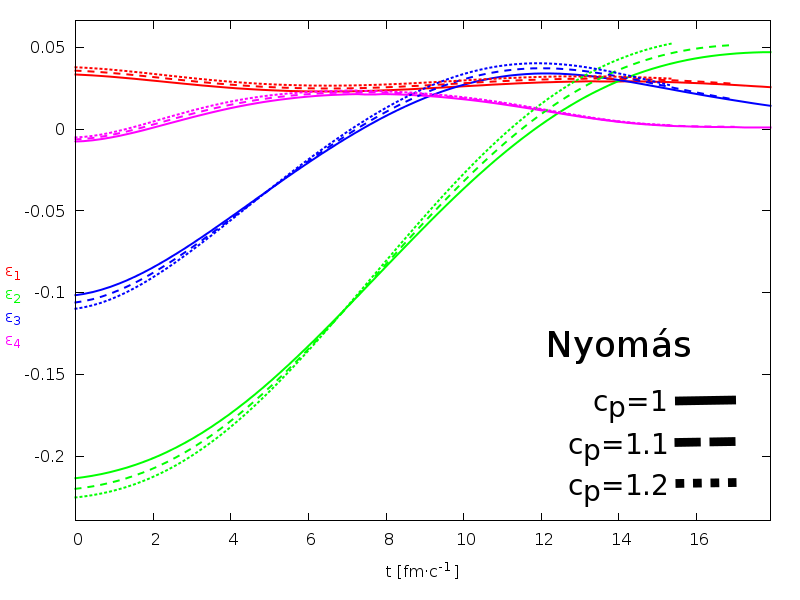
\includegraphics[width=\textwidth]{pic/res/rel/eps_pc_p}
	\end{subfigure}
	\begin{subfigure}[b]{0.49\textwidth}
        	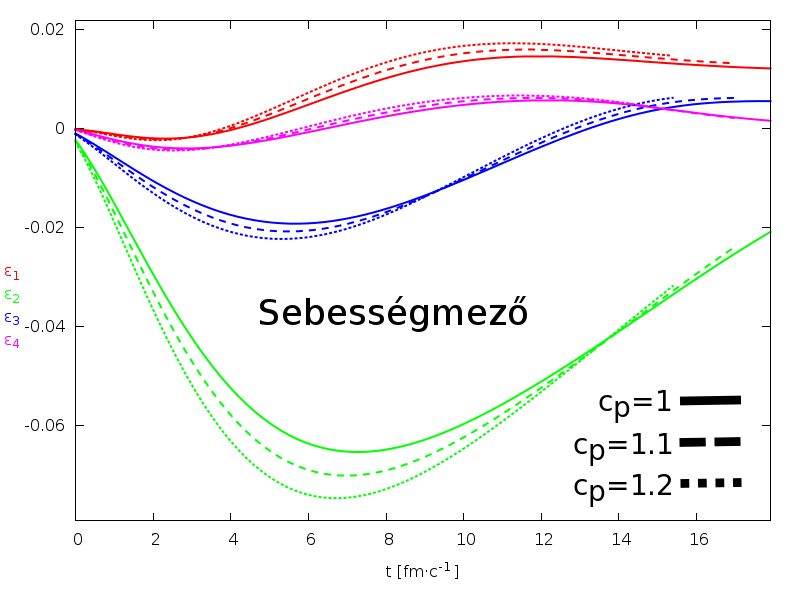
\includegraphics[width=\textwidth]{pic/res/rel/eps_pc_v}
	\end{subfigure}
\end{figure}
\end{center}
\end{frame}

\section{Relativisztikus és nemrelativisztikus hidrodinamika}
\subsection{Összehasonlítás}
\begin{frame}
\frametitle{Relativisztikus és nemrelativisztikus hidrodinamika összehasonlítása}
\begin{center}
\begin{itemize}
\setlength{\itemsep}{12pt}
\item<1-> Relativisztikus eset: lassabban tűnik el az asszimmetria
\item<1-> Nemrelativisztikus eset: sebességmezőben nagyobb aszimmetria alakul ki

\end{itemize}
\begin{figure}[H]
	\centering
    \begin{subfigure}[b]{0.49\textwidth}
    		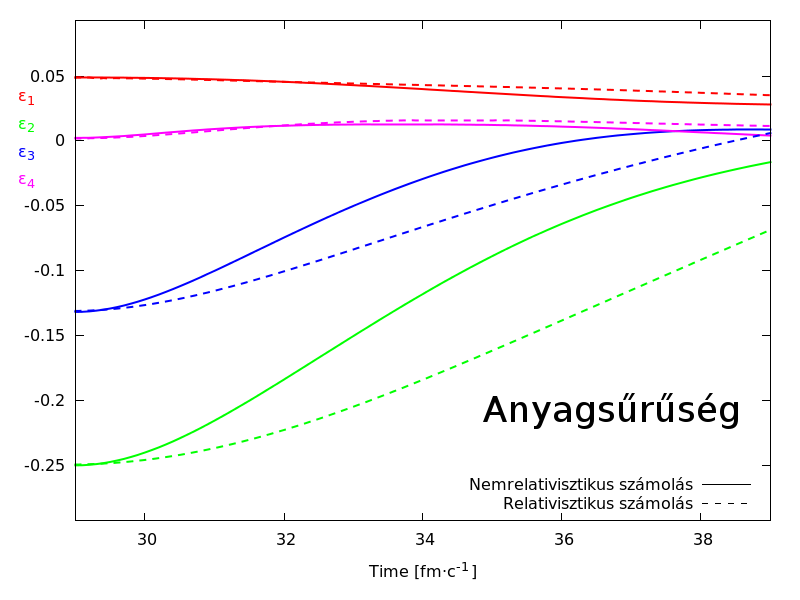
\includegraphics[width=\textwidth]{pic/res/relnonrel_n}
	\end{subfigure}
	\begin{subfigure}[b]{0.49\textwidth}
        	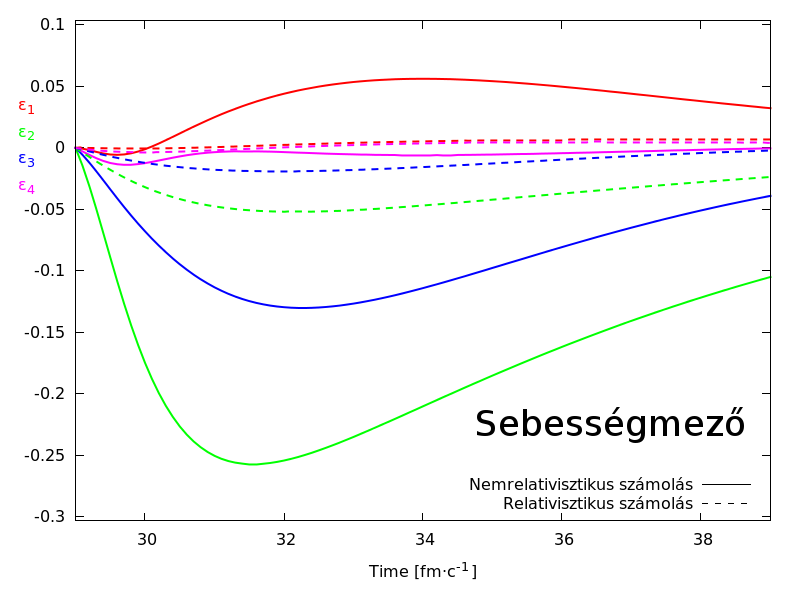
\includegraphics[width=\textwidth]{pic/res/relnonrel_v}
	\end{subfigure}
\end{figure}
\end{center}
\end{frame}

\section{Relativisztikus és nemrelativisztikus hidrodinamika}
\begin{frame}
\frametitle{Relativisztikus és nemrelativisztikus hidrodinamika összehasonlítása}
\begin{center}
\begin{figure}[H]
	\centering
    \begin{subfigure}[b]{0.49\textwidth}
    		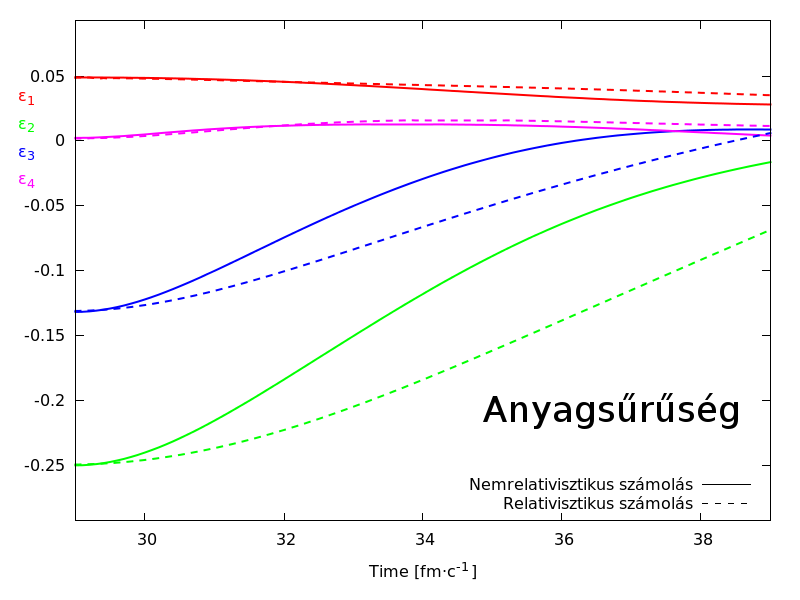
\includegraphics[width=\textwidth]{pic/res/relnonrel_n}
	\end{subfigure}
	\begin{subfigure}[b]{0.49\textwidth}
        	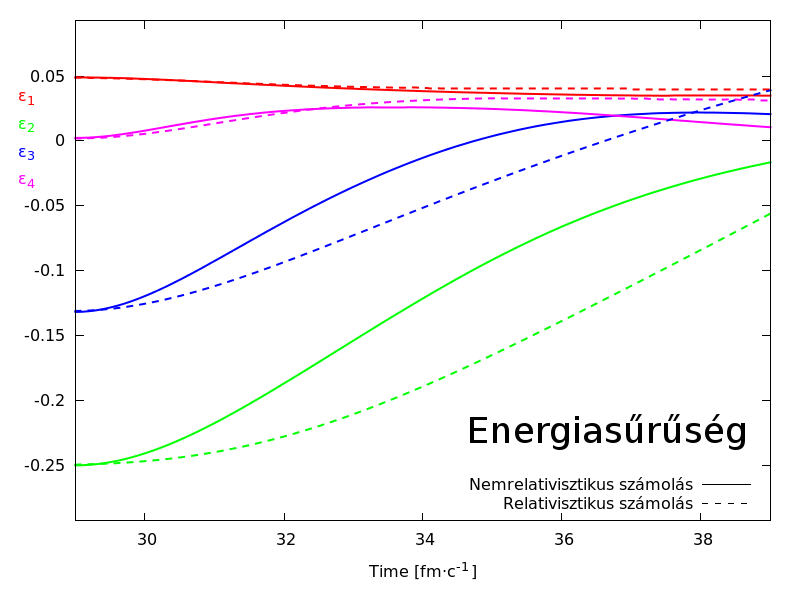
\includegraphics[width=\textwidth]{pic/res/relnonrel_e}
	\end{subfigure}
\end{figure}
\end{center}
\end{frame}


\subsection{Kifagyás}
\begin{frame}
\frametitle{Kifagyás}
\begin{itemize}
\item<1-> Hőmérséklet $\downarrow\;\;\;\Rightarrow$ kvark-szabadsági fokok eltűnnek $\Rightarrow$ hadronok
\item<1-> Maxwell-Jüttner típusú forrásfüggvény: 
$S(x, p)d^4x=\mathcal{N}n(x)\exp{\bigg(-\frac{p_\mu u^\mu}{T(x)}\bigg)}H(\tau)p_\mu d^3\frac{u_\mu d^3x}{u^0} d\tau$
\item<1-> Mérhető mennyiségek:
$v_n(p_t)=\langle\cos(n\varphi)\rangle_{N}=\frac{1}{N(p_t)}\int_0^{2\pi} N(p_t, \varphi)\cos(n\varphi)d\varphi$
\end{itemize}
\begin{minipage}{0.49\textwidth}
\begin{center}
\includegraphics<1->[scale=0.23]{pic/res/rel/vn_kappa}
\end{center}
\end{minipage}
\begin{minipage}{0.5\textwidth}
\begin{itemize}
\item<1-> Impulzustérbeli aszimmetriák: erősen függés a hangsebességtől
\item<1-> Hangsebességre érzékeny: kifagyás ideje
\end{itemize}
\end{minipage}
\end{frame}

\section{Összegzés}
\begin{frame}
\frametitle{Összegzés}
\begin{itemize}
\setlength{\itemsep}{16pt}
\item<1-> Motiváció: egyszerű effektusok, hogyan befolyásolják az aszimmetriák időfejlődését
\item<1-> Analitikus tárgyalás korlátozottabb, ezért numerikus módszert alkalmaztunk
\item<2-> Kezdőfeltétel hasonló a már létező analitikus megoldásokhoz, de realisztikusabb
\item<3-> A viszkozitás lassabbá teszi az anyag- és energiasűrűségben számolt aszimmetriák időfejlődését, sebességeloszlásban gyorsabbá
\item<4-> Hangsebesség csökkentése lassítja az aszimmetriák időfejlődését, kifagyás később következik be
\end{itemize}
\end{frame}

\section{}
\begin{frame}
\begin{center}
\textbf{\huge{Köszönöm a figyelmet!}}
\end{center}
\end{frame}




\subsection{Kifejlesztett kód tesztelése}
\begin{frame}[noframenumbering]
\frametitle{Kód tesztelése}
\begin{itemize}
  \setlength{\itemsep}{5pt}
\item<1| only@1> Nemrelativisztikus esetben: egzakt megoldással (Csörgő et al, PhysRevC67):

\begin{equation*}
s=\frac{x^2}{X^2(t)}+\frac{y^2}{Y^2(t)}
\end{equation*}

\begin{equation*}
\rho = \rho_0\frac{V_0}{V}e^{-s},\;\;\; p=p_0\bigg(\frac{V_0}{V}\bigg)^{1+\frac{1}{\kappa}}e^{-s}
\end{equation*}

\begin{equation*}
\bm{v}(t, \bm{r})=\bigg(\frac{\dot{X}}{X}x, \frac{\dot{Y}}{Y}y\bigg)
\end{equation*}

\begin{equation*}
\ddot{X}X=\ddot{Y}Y=\frac{T_i}{m}\bigg(\frac{V_0}{V}\bigg)^{\frac{1}{\kappa}},\;\;V=X(t)Y(t)
\end{equation*}
\end{itemize}
\end{frame}







\section{Nemrelativisztikus eredmények}
\subsection{Viszkozitás hatása}
\begin{frame}[noframenumbering]
\frametitle{Viszkozitás hatása: $\varepsilon_n$ anyag- és energiasűrűségben}
\begin{center}
\begin{figure}[H]
	\centering
    \begin{subfigure}[b]{0.49\textwidth}
    		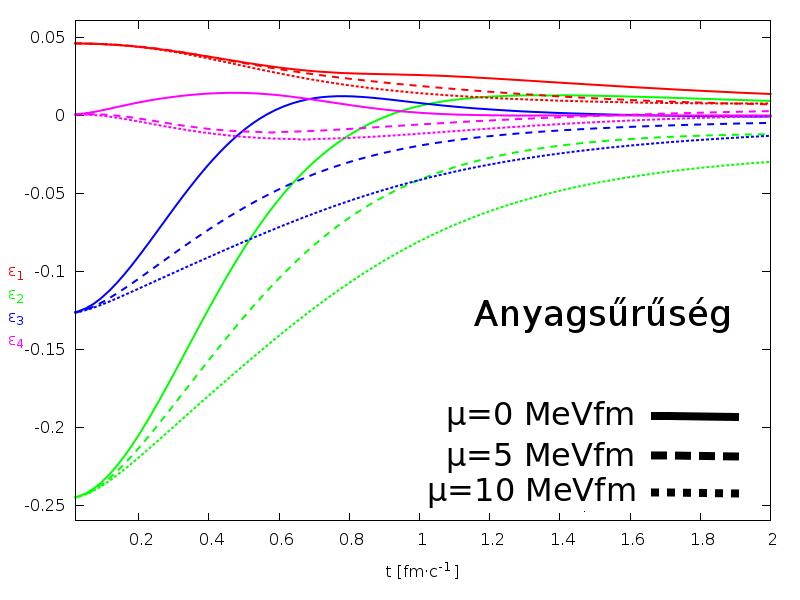
\includegraphics[width=\textwidth]{pic/res/nonrel/eps_visc_r}
	\end{subfigure}
	\begin{subfigure}[b]{0.49\textwidth}
        	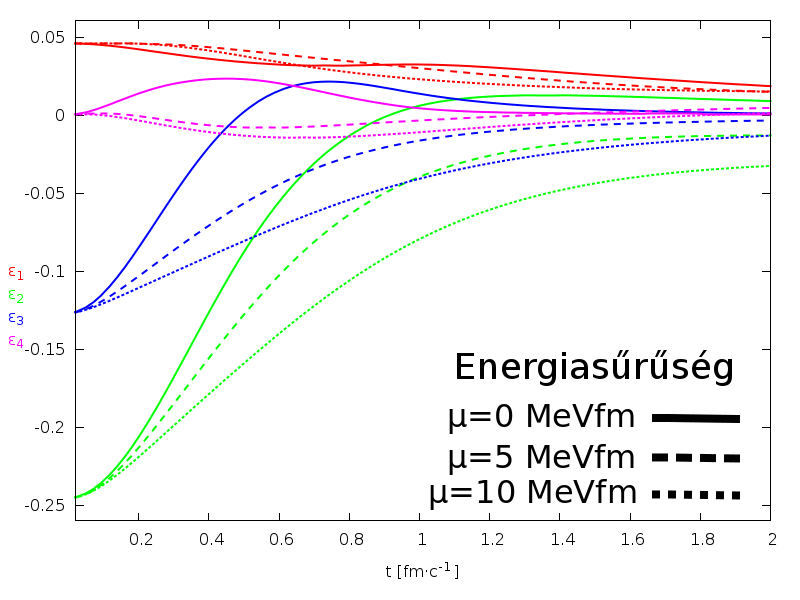
\includegraphics[width=\textwidth]{pic/res/nonrel/eps_visc_p}
	\end{subfigure}
\end{figure}
\end{center}
\end{frame}

\subsection{Hangsebesség hatása}
\begin{frame}[noframenumbering]
\frametitle{Hangsebesség hatása: $\varepsilon_n$ anyag- és energiasűrűségben}
\begin{center}
\begin{figure}[H]
	\centering
    \begin{subfigure}[b]{0.49\textwidth}
    		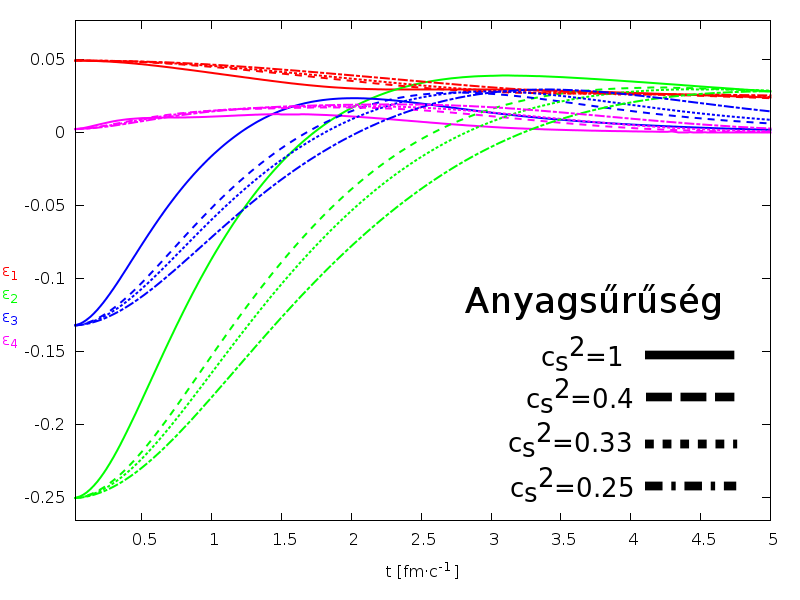
\includegraphics[width=\textwidth]{pic/res/nonrel/eps_cs2_r}
	\end{subfigure}
	\begin{subfigure}[b]{0.49\textwidth}
        	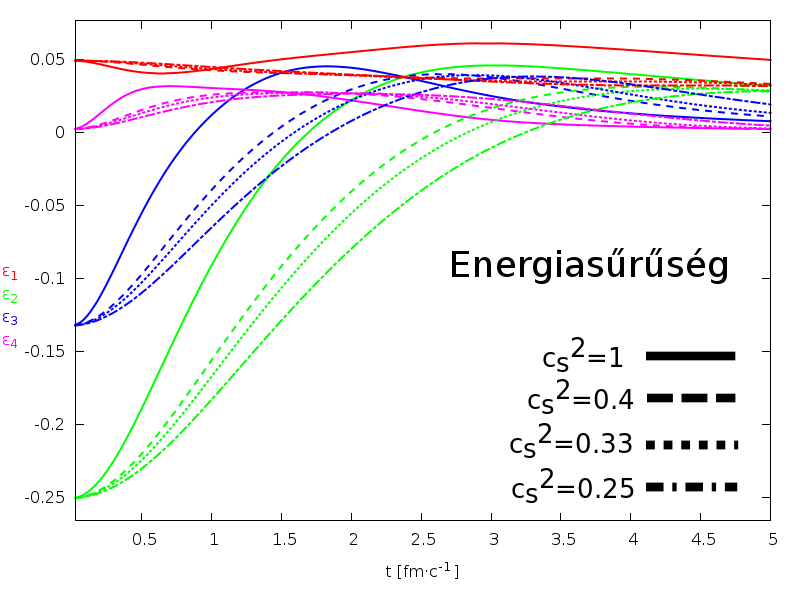
\includegraphics[width=\textwidth]{pic/res/nonrel/eps_cs2_p}
	\end{subfigure}
\end{figure}
\end{center}
\end{frame}

\subsection{Nyomásgradiens hatása}
\begin{frame}[noframenumbering]
\frametitle{Nyomásgradiens hatása: $\varepsilon_n$ anyag- és energiasűrűségben}
\begin{center}
\begin{figure}[H]
	\centering
    \begin{subfigure}[b]{0.49\textwidth}
    		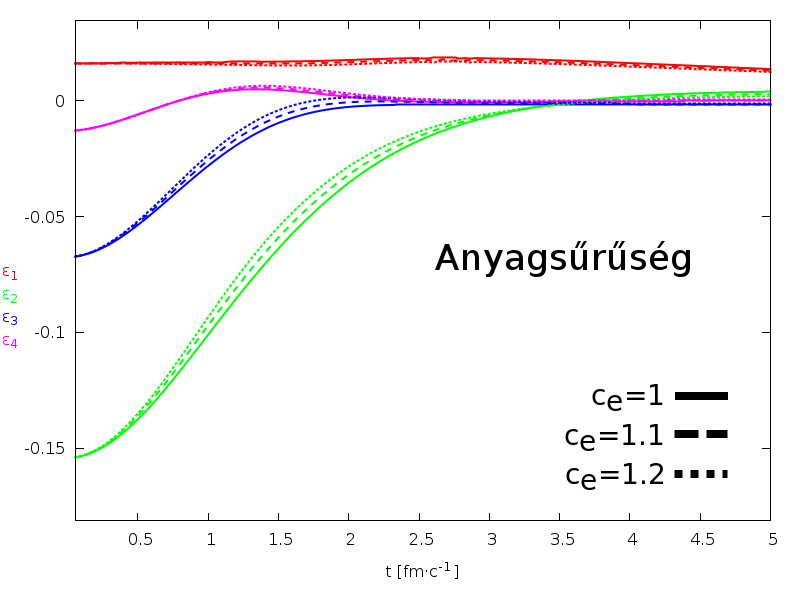
\includegraphics[width=\textwidth]{pic/res/nonrel/eps_ec_r}
	\end{subfigure}
	\begin{subfigure}[b]{0.49\textwidth}
        	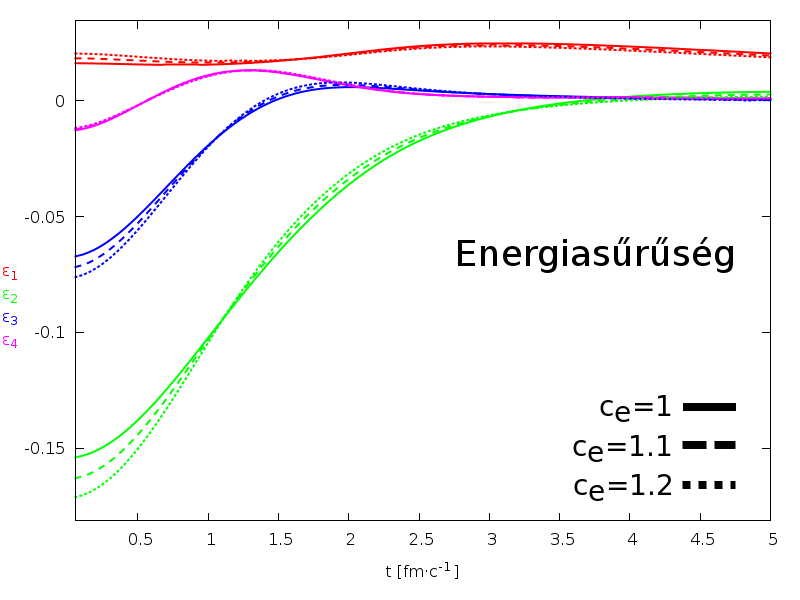
\includegraphics[width=\textwidth]{pic/res/nonrel/eps_ec_p}
	\end{subfigure}
\end{figure}
\end{center}
\end{frame}

\section{Relativisztikus eredmények}
\subsection{Hangsebesség hatása}
\begin{frame}[noframenumbering]
\frametitle{Hangsebesség hatása: $\varepsilon_n$ számsűrűségben és nyomáseloszlásban}
\begin{center}
\begin{figure}[H]
	\centering
    \begin{subfigure}[b]{0.49\textwidth}
    		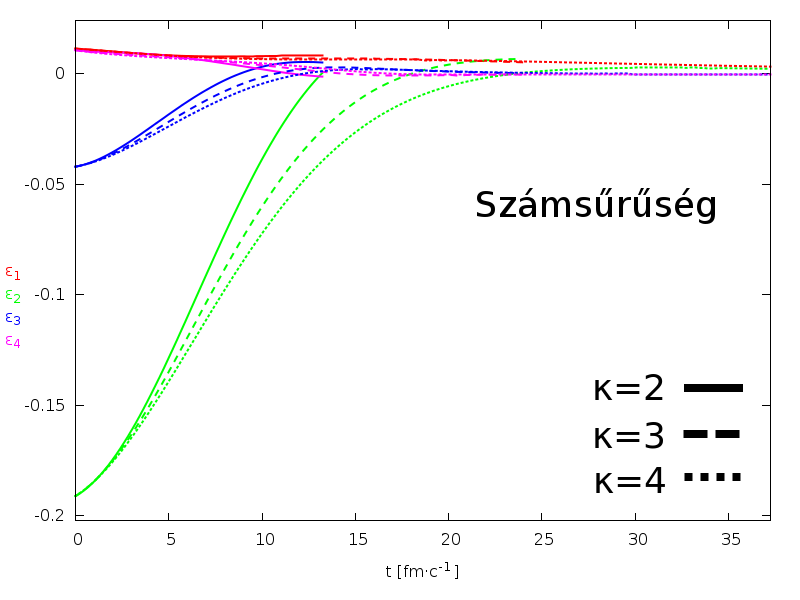
\includegraphics[width=\textwidth]{pic/res/rel/eps_kappa_n}
	\end{subfigure}
	\begin{subfigure}[b]{0.49\textwidth}
        	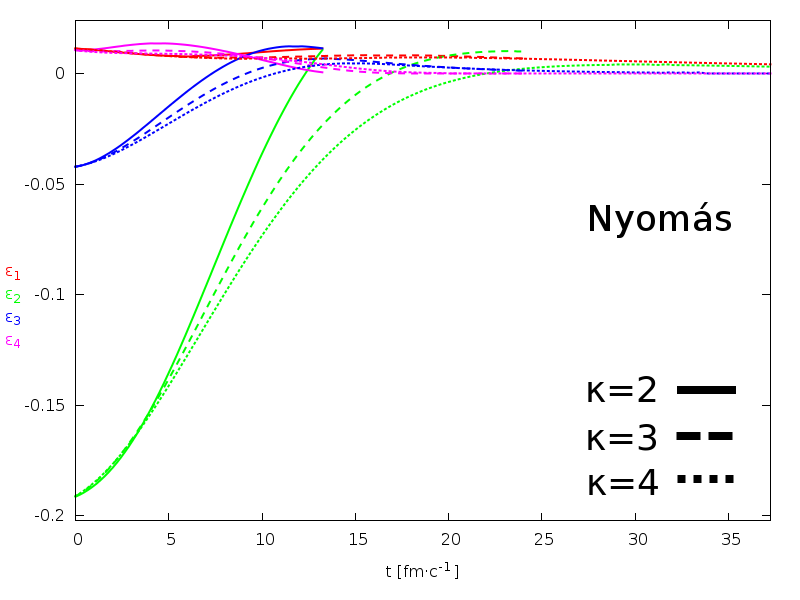
\includegraphics[width=\textwidth]{pic/res/rel/eps_kappa_p}
	\end{subfigure}
\end{figure}
\end{center}
\end{frame}

\subsection{Nyomásgradiens hatása}
\begin{frame}[noframenumbering]
\frametitle{Nyomásgradiens hatása: $\varepsilon_n$ számsűrűségben és nyomáseloszlásban}
\begin{center}
\begin{figure}[H]
	\centering
    \begin{subfigure}[b]{0.49\textwidth}
    		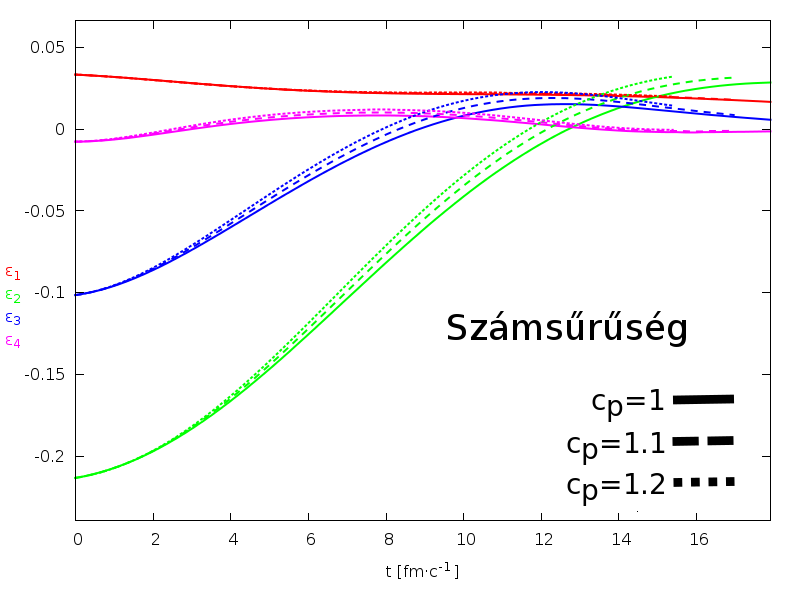
\includegraphics[width=\textwidth]{pic/res/rel/eps_pc_n}
	\end{subfigure}
	\begin{subfigure}[b]{0.49\textwidth}
        	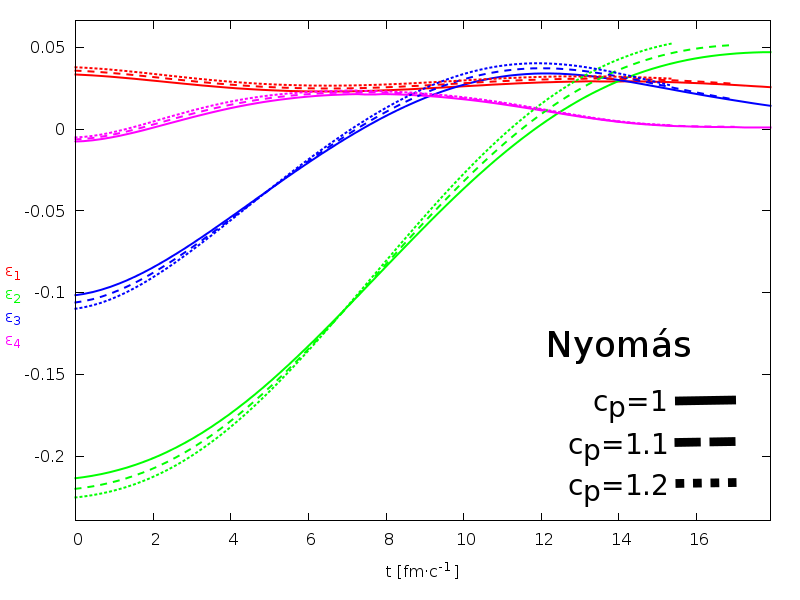
\includegraphics[width=\textwidth]{pic/res/rel/eps_pc_p}
	\end{subfigure}
\end{figure}
\end{center}
\end{frame}

\section{Kitekintés}
\begin{frame}[noframenumbering]
\frametitle{Kitekintés}
\begin{itemize}
\setlength{\itemsep}{20pt}
\item<1-> Viszkozitás hatásának vizsgálata relativisztikus esetben
\item<1-> Relativisztikus és nemrelativisztikus viszkozitás összehasonlítása
\item<1-> QCD állapotegyenlet használata
\end{itemize}
\end{frame}


\end{document}

